\newpage
\section{提案手法}
本研究では,ハードウェア特徴点の採取システムを構築し,\fp~により端末構成を推定することを試みた.
これは既存の\fp~とは異なり,端末やブラウザを識別するだけではなく,端末がどのハードウェアで構成されているのかを明らかにするものである.
よって,ここでは新たに\hfp~という用語でこの手法を取り扱うこととする.
また,新たなハードウェア特徴点の採取法についても提案する.

\subsection{\hfp}
本研究では,\hfp~を\fp~を拡張して,``ブラウザ経由で採取したFingerprintにより端末の構成要素(ハードウェア)を識別する''と定義する.
\hfp~では,基本的に図~\ref{fig-hfp}で示すフローで推定を行う.これは一般的な教師あり学習であり,学習フェーズにてJavaScriptによる特定の演算結果をハードウェア情報でラベル付し教師データとする.そして,推定フェーズにて同様のJavaScriptによる演算を行った結果,教師データを参照して最も近しいラベルを推定結果とするものである.ここで重要なことは,教師データの確保である.すべてのハードウェアを推定するためには多くのハードウェア上で実行された演算結果があることが望ましい.また,ラベル付されたデータに統計的ではない間違いが存在すると著しく推定確度が低下することに留意しなくてはならない.
\begin{figure}[H]
	\centering
    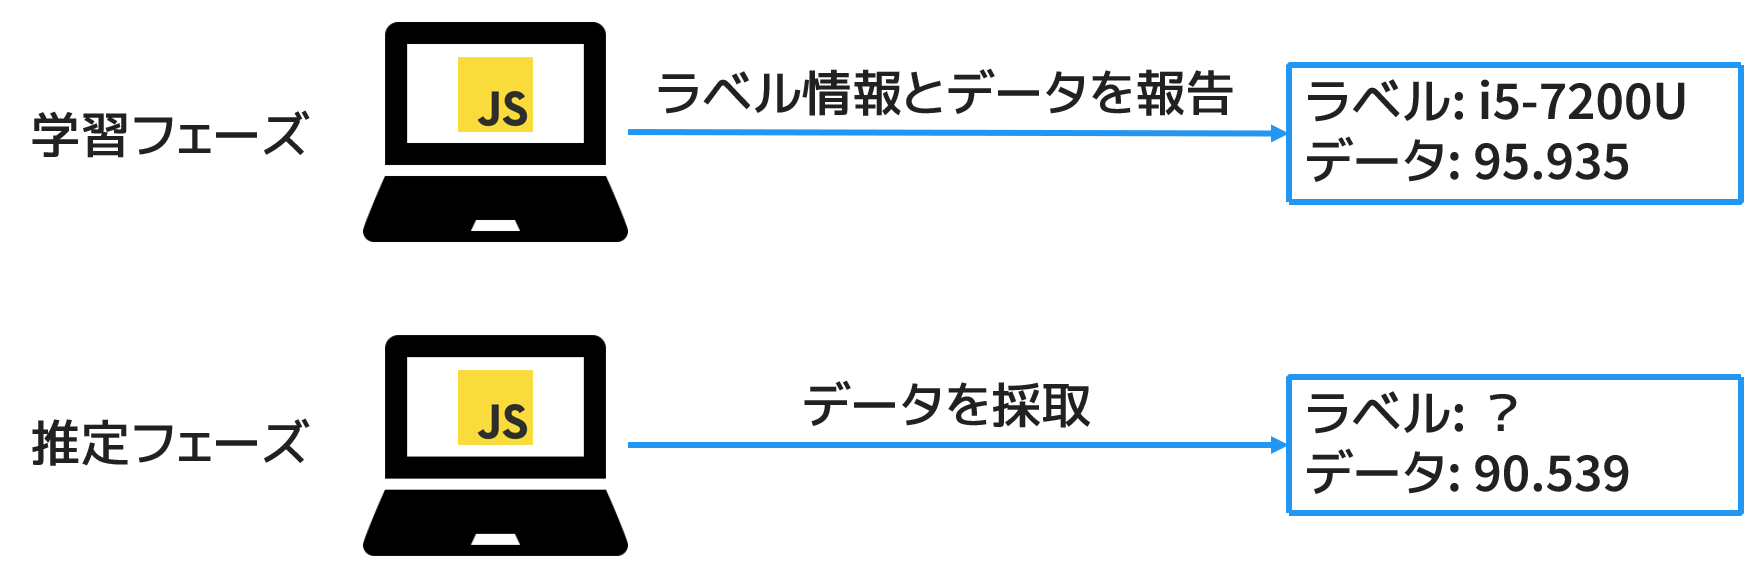
\includegraphics[width=\textwidth,pagebox=artbox]{fig/hfp.png}
    \caption{\hfp~の基本的なフロー}
    \label{fig-hfp}
\end{figure}

\subsection{\hfp~採取システム}
\hfp~採取システムは,WindowsとmacOSを対象に,SMBIOSに基づくBIOS情報をデータベースに送信するツールであるHardware Information Report ToolとHardware Fingerprintingを実施するWebサイトであるHardware Fingerprinting Siteから構成されている.
この採取システムでは新たに提案するハードウェア特徴点の中でもSMBIOSとの比較が行え,かつ実行時間が短いものを扱っている.
採取システムの実行フローを図\ref{fig-hfp_system}に示す.

\begin{figure}[H]
	\centering
    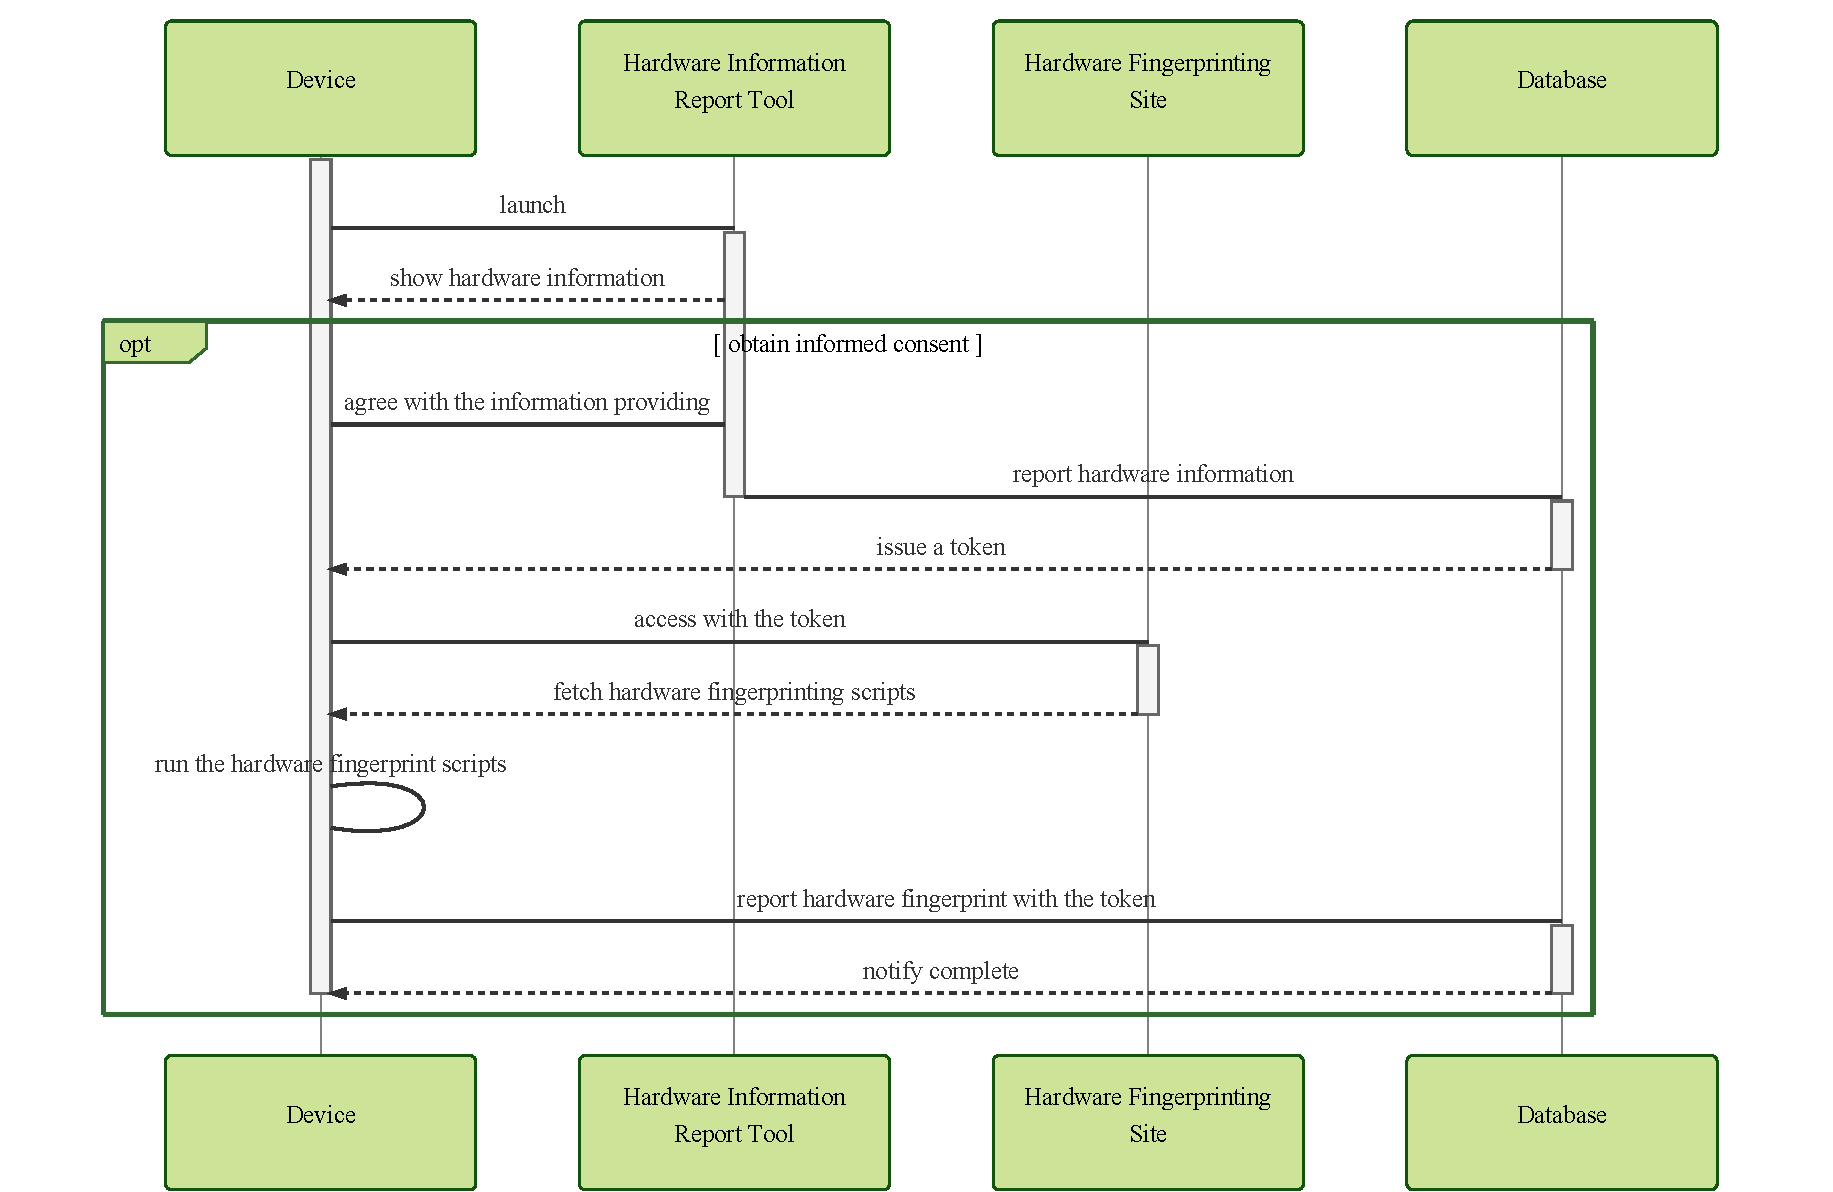
\includegraphics[width=\textwidth,pagebox=artbox]{fig/hero.pdf}
    \caption{\hfp~採取システムの実行フロー}
    \label{fig-hfp_system}
\end{figure}

採取は次の手順で行われる.

\begin{enumerate}
\item ユーザは端末上でHardware Information Report Toolを起動する.Hardware Information Report Toolには採取する情報と情報提供に同意するかについての文言が表示される.
\item ユーザが情報提供に同意する場合は署名をフォームに入力し,その後情報がデータベースに送信される.
\item 情報の送信が完了すると,自動的にブラウザが起動する.このとき,アクセスするURLはHardware Fingerprinting Siteのものであり,ユーザを識別するための一意なトークンがクエリパラメータとして付与されている.
\item Hardware Fingerprinting SiteではJavaScriptのプログラムを実行し,\hfp~を実施する.
\item プログラムの実行が完了すると,情報がデータベースに送信される.
\end{enumerate}
本節では実験システムを構成するそれぞれについて説明を行う.

\subsubsection{Hardware Information Report Tool}
Hardware Information Report Tool~\footnote{開発工程ではrSMBIOS (Reporting SMBIOS)と命名している.}は採取したSMBIOSをデータベースに送信する.
プログラムは起動するとSMBIOSを表示し,ユーザが情報提供に同意された場合のみ情報をデータベースに送信する.
情報が正常にデータベースに送信されると一意なトークンが発行される.
その後,プログラムは自動でブラウザを起動し,Hardware Fingerprinting Siteに,一意なトークンをURLパラメータに付与してアクセスする.

図~\ref{fig-rsmbios}にHardware Information Report Toolの外観を示す.

\begin{figure}[H]
	\centering
    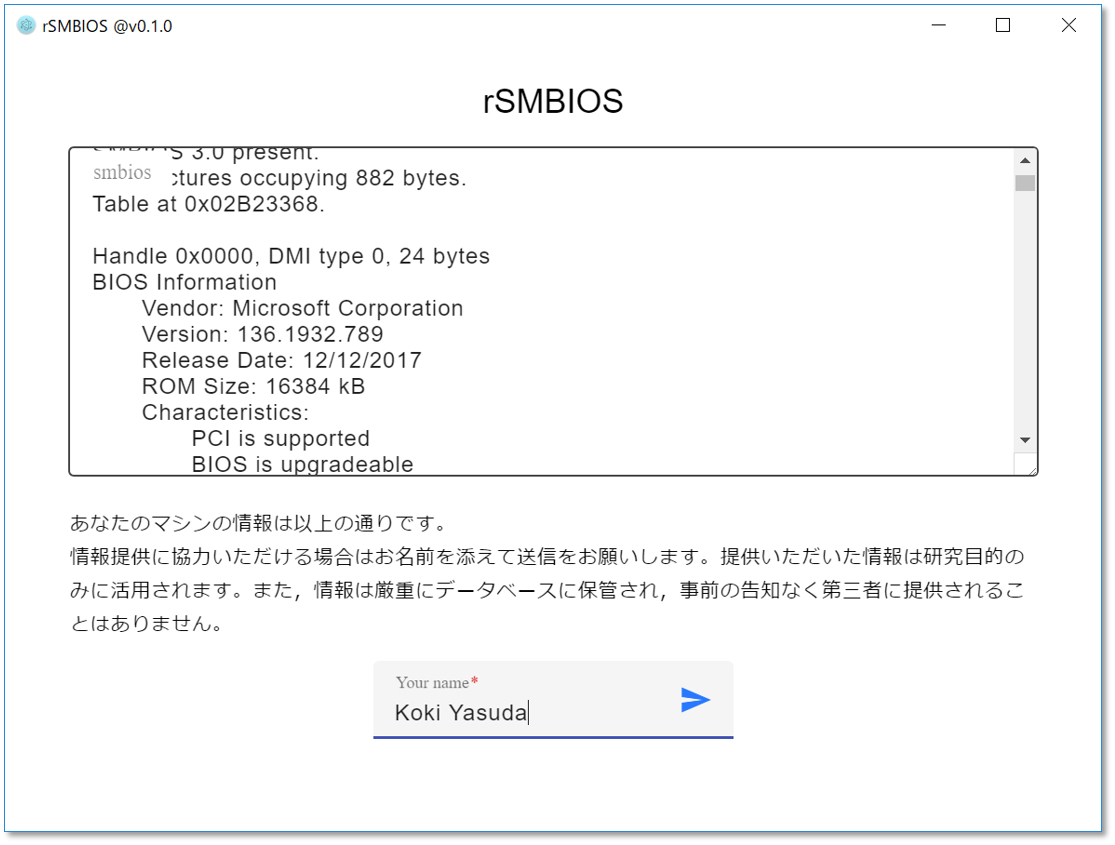
\includegraphics[width=\textwidth,pagebox=artbox]{fig/rsmbios.png}
    \caption{Hardware Information Report Toolの外観}
    \label{fig-rsmbios}
\end{figure}

採取する情報と情報提供に同意するかついての文言が確認できる.
実験においてはこの文言に同意し,署名したユーザのデータのみを収集している.

\subsubsection{Hardware Fingerprinting Site}
Hardware Fingerprinting SiteではHardware Information Report Toolの送信が完了した後に自動で起動するブラウザからアクセスされる.
このとき起動するブラウザはOSでURLを開く際に関連付けられたアプリケーションである.
これは一般的に,ユーザが普段のブラウジングに用いるものと同一である.

ここでは,次に示す端末構成を推定するためのJavaScriptのプログラムが実行される.
コードの全容については~\ref{cd-hfp}を参照されたい.

\begin{description}
	\item[OS]\mbox{}\\
   	\texttt{Math.tan(-1e300)}の演算誤差を利用する~\cite{tor_mathtan}
    \item[CPUのコア数,スレッド数]\mbox{}\\
    複数の\texttt{Web Worker}の処理速度比を利用する~\cite{後藤浩行2013web,桐生直輝2014web}
    \item[AES-NI]\mbox{}\\
    Web cryptography APIとそれ以外の演算との速度比を利用する
    \item[バイトオーダー]\mbox{}\\
    \texttt{Typed Array}の\texttt{DataView}がネイティブに依存することを利用する
    \item[メモリのパフォーマンス]\mbox{}\\
    \texttt{Typed Array}で保存される値がメモリに直に書き込まれることを利用する
    \item[GPU]\mbox{}\\
    WebGLの\texttt{WEBGL\_debug\_renderer\_info}から採取する~\cite{mowery2012pixel}
    \item[GPUのパフォーマンス]\mbox{}\\
    WebGLのシェーダを応用したGPGPUによるCPUとの演算速度比を利用する
\end{description}

プログラムの実行が完了すると,アクセスの際に付与されている一意なトークンとともに採取した情報をデータベースに送信する.

\subsection{新たなハードウェア特徴点}
本節では,新たなハードウェア特徴点の採取法を提案する.
ここで扱う特徴点の一部は,先に示した\hfp~採取システムに実装されている.

\subsubsection{AES-NI}
AES-NIはAESの暗号化,復号処理を高速化する.
この機能はCPU命令の一種であり,CPUの種類によっては搭載されていないことから,命令の有無を判別できればCPUの推定に活用することができる.
図~\ref{fig-aes_ni}にAES-NIのベンチマークをAES-NIが有効でない場合との比較結果を示す.
これは,OpenSSLの\texttt{openssl speed aes}で取得した結果を参考にしている.

\begin{figure}[H]
	\centering
    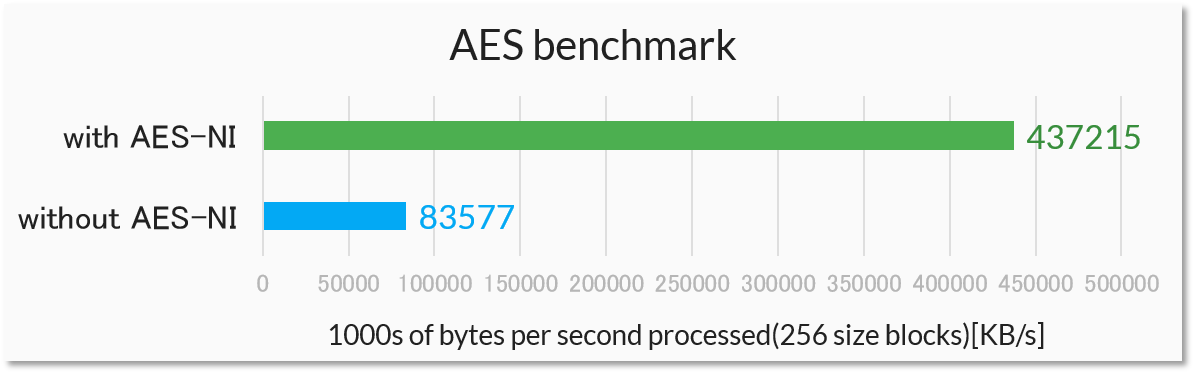
\includegraphics[width=\textwidth,pagebox=artbox]{fig/aes_ni.png}
    \caption{AES-NIのベンチマーク}
    \label{fig-aes_ni}
\end{figure}

図からも分かる通り,AES-NIが有効の場合はそうでない場合よりも,一般的に3倍から10倍程度処理を高速化することができる.

AES-NIをブラウザで活用するためにはWeb Cryptography API~\cite{web_crypto}を使用する.
このAPIによるAESの処理を行うことで,AES-NIが有効な端末と無効な端末の演算速度に差が生じると考えられる.
ただし,CPUの基本的な演算速度は性能により異なるので,AES-NIに関係なく処理時間に違いが出てしまう.
そこで,AES-NIに依存しない演算速度の基準となる処理時間でAESの処理時間を正規化する.
AES-NIが無効の場合は,演算の基準となる処理とAESの処理時間は同程度の演算速度になる.
一方,AES-NIが有効の場合,演算の基準となる処理と比較してAESの処理時間は短くなる.

AES-NIに依存しない演算にはモンテカルロ法による円周率$\pi$の演算を使用した.
AES-NIを推定するために必要な演算式は以下の通りになる.

\begin{eqnarray*}
  AESRate = \frac{the\ time\ of\ AES\ operation}{the\ time\ of\ Monte\ Carlo\ calculation}
\end{eqnarray*}

AES-NIが有効な端末は,AES-NI無効もしくは非搭載のものよりAESRateが小さくなる傾向になる.
AESを用いた処理 (AES operation) はWeb Cryptography APIを用いて,暗号モードAES-CBC,鍵長128ビットで整数配列の暗号化と復号を64,000,000回繰り返した.
AES-NIに依存しない演算 (Monte Carlo calculation) はモンテカルロ法を用いて,円周率の演算を50,000,000回繰り返した.
以上の演算を1セットとし,これを10セット行い,平均値を処理時間とし,AESRateの算出を行った.

\subsubsection{Turbo Boost}
Turbo BoostはCPUで処理するすべての演算に対して動作するので,演算の基準となる処理が存在しない.
しかし,Turbo Boostは負荷が高い処理などに対して効果的に機能しないことが知られているので,処理内容によって処理速度に違いが生じる可能性がある.
そこで,処理内容に対してTurbo Boostがどの程度機能するかを確認するためにJavaScriptベンチマークソフトであるOctane 2.0~\footnote{Googleが開発したJavaScriptベンチマークソフト.\url{https://developers.google.com/octane/}}を用いてTurbo Boost有効時と無効時の処理能力の変化を調査した.
Octane 2.0は17の項目についてベンチマークを測定することでJavaScriptの処理能力をスコアとして表すことができる.

事前検証として,Turbo Boost有効時と無効時のそれぞれ20回測定したベンチマークを図~\ref{fig-turbo_boost}に示す~\footnote{検証環境は,Windows10,Intel(R) Core(TM) i5-4300U,8GB,Chrome47.0である.}. 

\begin{figure}[H]
	\centering
    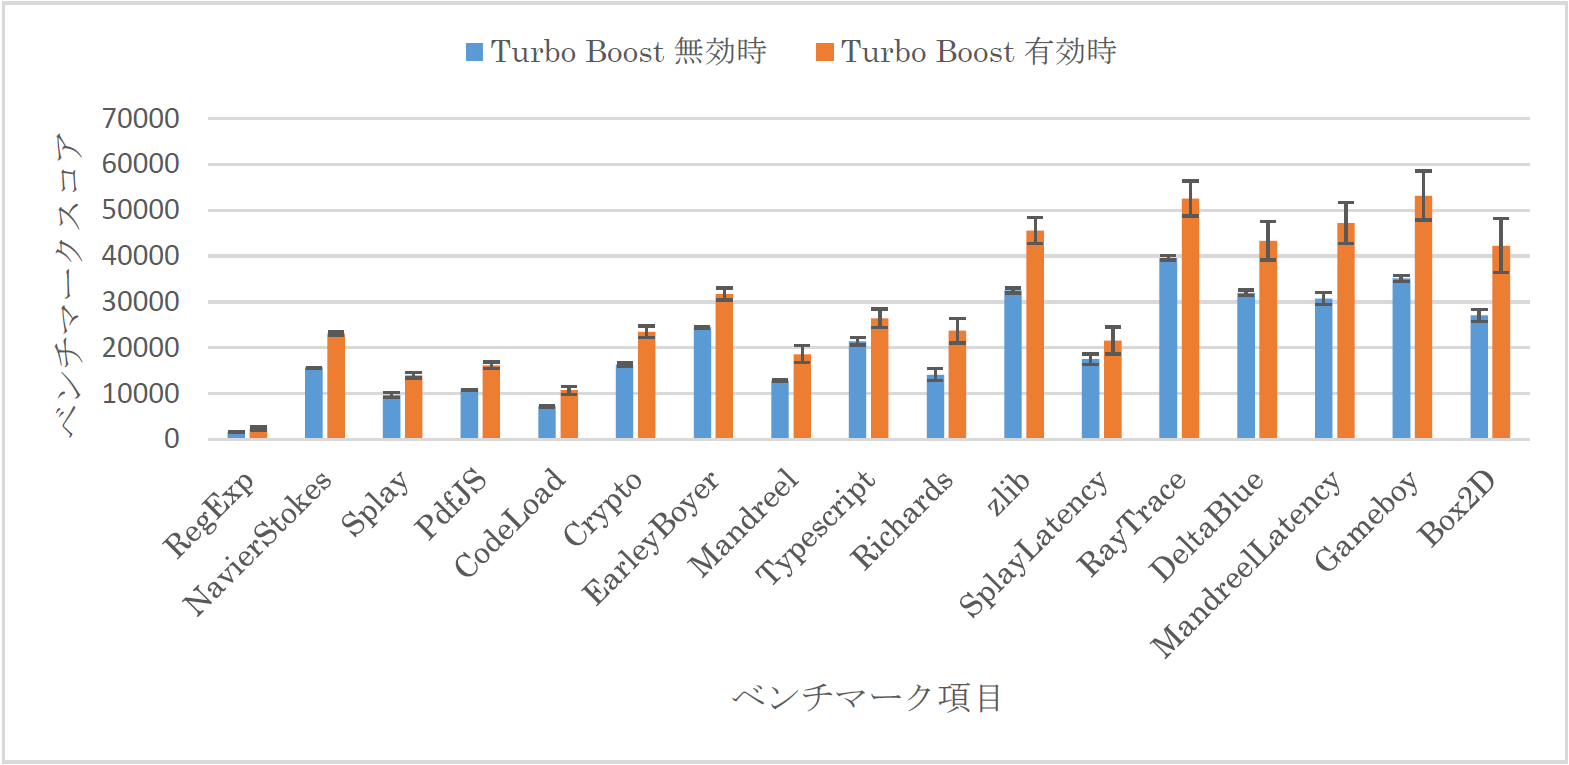
\includegraphics[width=\textwidth,pagebox=artbox]{fig/turbo_boost.png}
    \caption{Turbo Boostのベンチマーク}
    \label{fig-turbo_boost}
\end{figure}

ベンチマークスコアは値が大きいほど性能が良いことを表し,ベンチマーク項目は標準偏差が小さい順にソートしてある.
ここで,ベンチマークスコアはノイズなどのTurbo Boost以外の要因により変動するので,標準偏差の小さい項目のみに注目する.

RegExpのTurbo Boost無効時の平均スコアは1638,有効時の平均スコアは2353となった.
また,NavierStokesのTurbo Boost無効時の平均スコアは15678.7,有効時の平均スコアは23091となった.
RegExpのTurbo Boostの有無による比率は1.437,NavierStokesの比率は1.4727であり,Turbo Boostの効果は処理内容に応じて変化することが分かった.

推定を行う際には$\frac{NavierStokes}{RegExp}$を算出する.
この事前検証では,Turbo Boost無効時は9.572,有効時は9.813となり,Turbo Boost無効時と有効時で異なる値を示すことがわかる.
Turbo Boostの有無もしくは搭載・非搭載は,この比率を利用することで推定が可能となる.

\subsubsection{CPUファミリ,マイクロアーキテクチャ,モデルナンバー}
CPUの推定は次のフローで行われる.

\begin{enumerate}
\item CPU機能による絞り込み.SSE2,物理コア数,HTT,AES-NIによって推定対象を絞り込む.
\item CPUパフォーマンスによる推定.JavaScriptベンチマークを実行し,教師データに近しいCPUを推定結果とする.
\end{enumerate}

まず,CPU機能により推定対象を絞り込む.
\ref{tb-cpu}にCPUファミリごとの機能の差異を示している.
ここから,CPUの機能が判明すれば,CPUファミリやマイクロアーキテクチャ,モデルナンバーの絞り込みが行えることが分かる.
例えば,SSE2が有効,物理コア数が2,HTTが有効,AES-NIが有効の場合は図~\ref{fig-cpu_est}における緑で着色した部分に該当することが分かる.
なお,図~\ref{fig-cpu_est}は\ref{tb-cpu}から一部抜粋したものである.

\begin{figure}[H]
	\centering
    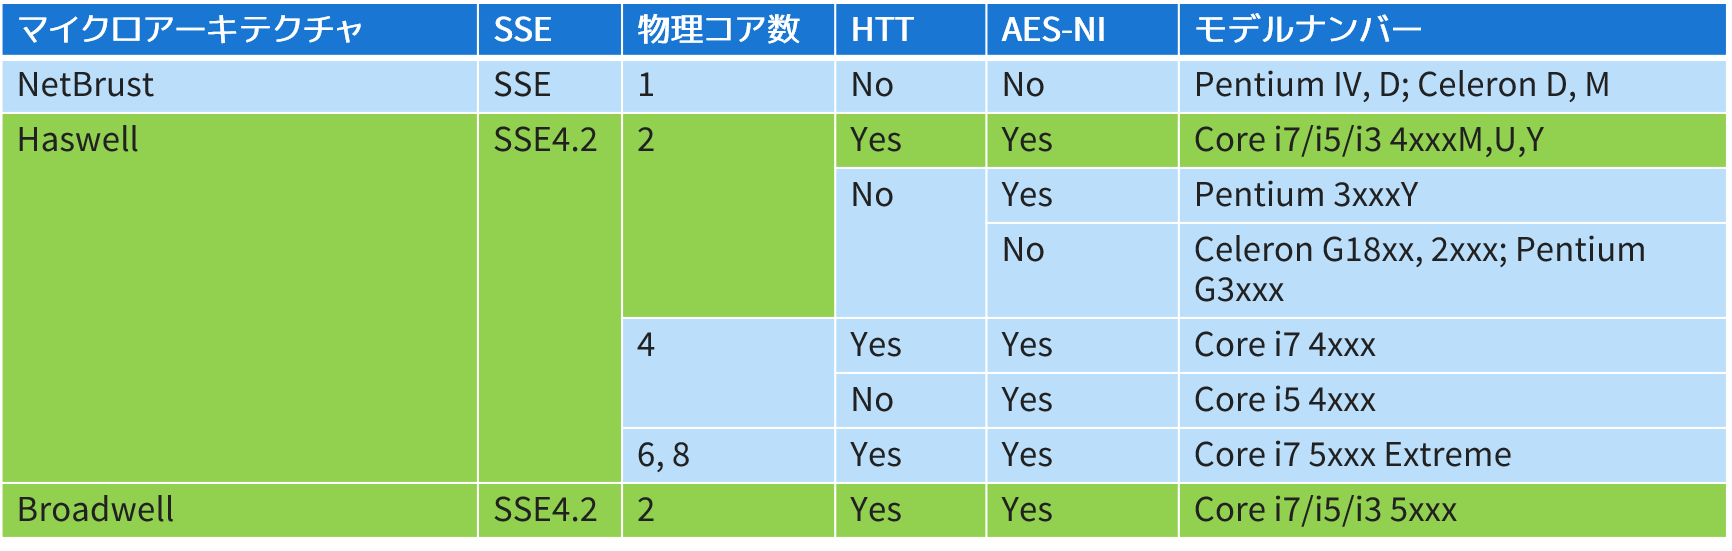
\includegraphics[width=\textwidth,pagebox=artbox]{fig/cpu_est.png}
    \caption{CPU推定の絞り込みのフロー}
    \label{fig-cpu_est}
\end{figure}

次に,CPUごとに演算パフォーマンスが異なることから,JavaScriptベンチマークによる推定を行う.
JavaScriptベンチマークにはOctane 2.0,SunSpider~\footnote{AppleのWebkitチームが開発したベンチマークソフト.\url{https://webkit.org/perf/sunspider/sunspider.html}},Kraken~\footnote{Mozillaが開発したベンチマークソフト.\url{https://krakenbenchmark.mozilla.org/}}を用いた.
また,ブラウザファミリによって基本的な演算速度に差異があることから,ブラウザファミリに応じて教師データを分割している.
推定の際は,1-nearest neighbor algorithmを用いた.
これは,最も近しい教師データを推定結果とする,単純なアルゴリズムである.

\subsubsection{バイトオーダー}
JavaScriptには効率的にバイナリデータを扱う必要性から\texttt{Typed Array}が実装されている.
バッファとビューに実装が別れており,バッファにあるデータにアクセスするにはビューを使用する.
ビューには\texttt{Int8}や\texttt{Uint32}など数値型に応じた種類があり,対応する数値型でバッファのデータを読み書きする.
このときビューはネイティブのバイトオーダーとなる.コード~\ref{cd-endian}にバイトオーダーの採取に用いたコードを示す.

\lstinputlisting[caption=バイトオーダー,label=cd-endian,language=JavaScript]{code/endian.js}

\texttt{Uint16Array}で確保したメモリはネイティブのバイトオーダーに応じてメモリに確保される.
確保されたメモリ領域を\texttt{Uint8Array}で読み取ったときに,バイトオーダーに応じて値が変化する.
コード~\ref{cd-endian}にコードはリトルエンディアンのときに\texttt{true}を返す.

\subsubsection{メモリのパフォーマンス}
\texttt{Typed Array}はメモリを直接参照できることから,\texttt{Typed Array}を用いたアクセスのパフォーマンスを計測する.
推定に用いたコードをコード~\ref{cd-memory}に示す.

\lstinputlisting[caption=メモリのパフォーマンス,label=cd-memory,language=JavaScript]{code/memory.js}

まず,適当なサイズの\texttt{Array Buffer}を確保した後に数値を書き込み初期化する.
次に現在時刻を\texttt{t0}とし,\texttt{TypedArray.prototype.reverse()}で書き込んだ数値を反転させる.
\texttt{TypedArray.prototype.reverse()}は読み書きを同時に実施することから選出した.
処理が終わったときの現在時刻と\texttt{t0}を比較し処理時間を計測する.
これを最初に確保するサイズを変化させながら,処理時間の比率を算出する.

\subsubsection{GPUのパフォーマンス}
WebGLはWebにおいてグラフィックスのレンダリングを行うAPIである.
WebGLの実行にはJavaScriptコードだけではなく,GLSLで記述されるシェーダプログラムが必要である.
シェーダプログラムはGPUによって実行され,並列計算を実行することでCPUよりも効率的な演算が可能である.
また,データを画像として符号化し任意の計算を実行させることもできる.
この際,テクスチャに読み書きを行うことで実際に画面に描画されることはない.
このようにレンダリングのみにGPUを使用せずに汎用的な計算をさせる利用法はGPGPUと呼ばれている.

事前検証として,GPUありの場合の演算と,GPUなしの場合の演算を実施した~\footnote{GPUありはi7-4770+GTX660,GPUなしはGPUありの場合からGTX660を取り外して計測した.}
図~\ref{fig-gpgpu}に結果を示す.

\begin{figure}[H]
	\centering
    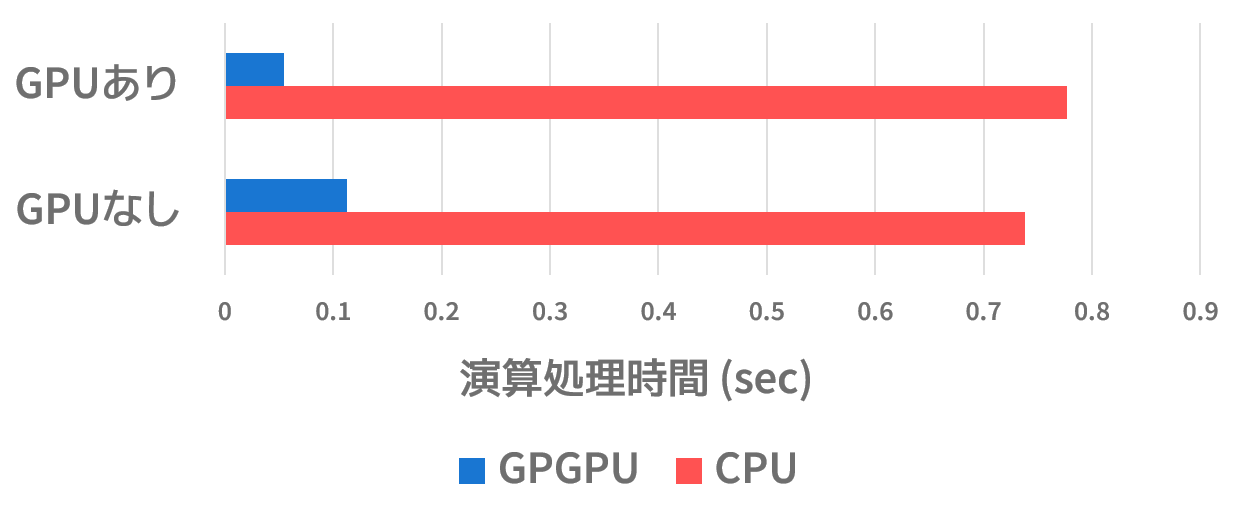
\includegraphics[width=\textwidth,pagebox=artbox]{fig/gpgpu.png}
    \caption{GPGPUのベンチマーク}
    \label{fig-gpgpu}
\end{figure}

GPUありの場合は,GPGPUとCPUの演算比が14.06となり,GPUなしの場合は6.54となった.
これにより,GPGPUを実施する際にGPUの存在が大きな影響を与えることがわかった.

つまり,端末に搭載されたGPUの性能に応じてGPGPU処理におけるパフォーマンスも向上する.
GPGPUパフォーマンスを測定することでGPU性能の傾向を推定することは可能といえる.
実装についてはgpu.js~\footnote{\url{http://gpu.rocks/}}を用い,GPGPUと同一の演算をCPUで行ったときの時間比率を計測した.
なお,Internet Explorerについては実行に必要なAPIであるWebGL 2.0が未実装であることから実行ができない.